\section{Results}

\begin{frame}{Fitness Evolution Across the Curriculum}
	The fitness graph clearly shows the impact of our curriculum learning.
	
	\begin{figure}
		\centering
		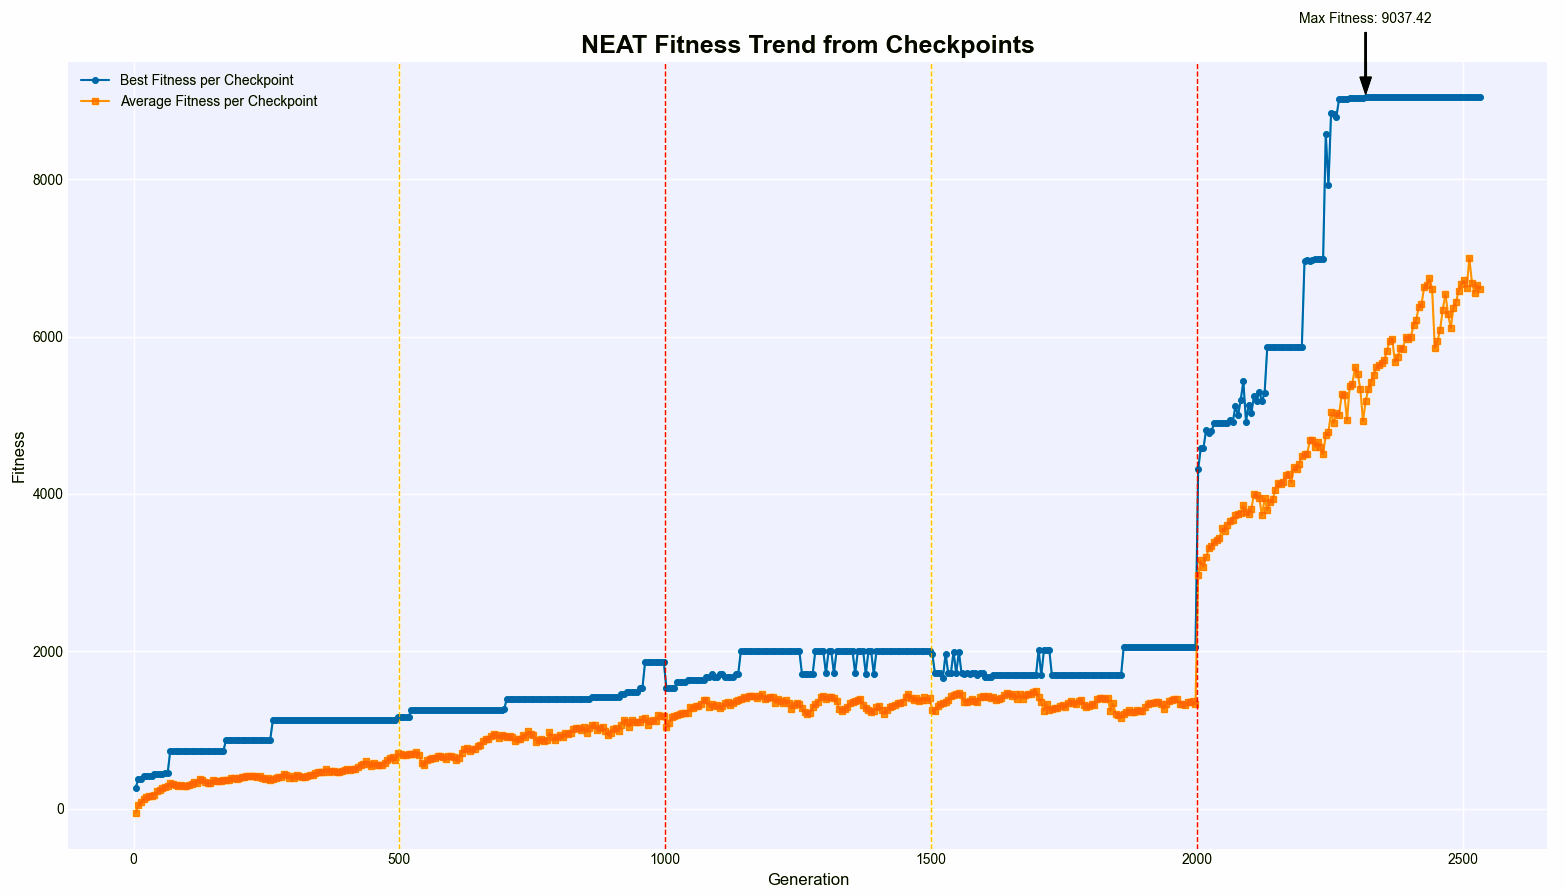
\includegraphics[width=\linewidth]{assets/fitness.png}
		\vspace{-2em}
		
		\caption{Best fitness per generation. Vertical lines mark curriculum phases.}
	\end{figure}
\end{frame}

\begin{frame}{Analysis of Emergent Behaviors}
	Analysis of the top-performing agents across curriculum phases reveals a progression in strategy:

	\textbf{Early Generations (Exploration)}
	\begin{itemize}
		\setlength\itemindent{-1em}
		\item Agents acquire basic \bfit{navigation skills}.
		\item Tend to become \bfit{stuck against walls} or exhibit \bfit{oscillatory behavior}.
	\end{itemize}

	\textbf{Mid Generations (Evasion)}
	\begin{itemize}
		\setlength\itemindent{-1em}
		\item Agents begin to \bfit{evade ghosts}, despite little improvement in fitness.
		\item The transition to scatter mode represents the most challenging phase due to \bfit{stochasticity}.
	\end{itemize}
	
	\textbf{Late Generations (Full Game)}
	\begin{itemize}
		\setlength\itemindent{-1em}
		\item Agents gradually adapt to the revised reward structure.
		\item Demonstrate \bfit{improved ghost avoidance} compared to earlier phases.
		\item Continue to \bfit{struggle with effective use of power-ups}.
	\end{itemize}
\end{frame}

\begin{frame}{The Best Genome in Action}

	A demonstration of the final agent's performance, showcasing its ability to navigate, evade, and clear the majority of the level.

	\begin{center}
		\begin{tikzpicture}
			\node[inner sep=0pt] (img) {\includegraphics[width=0.7\linewidth]{assets/thumbnail.png}};
			\node at (img.center) {
				\href{https://streamable.com/klb2iw}{
					\begin{tikzpicture}
						% Make the triangle longer and larger
						\filldraw[fill=gray, opacity=0.7, draw=none] (0.7,0) -- (-0.5,0.5) -- (-0.5,-0.5) -- cycle;
					\end{tikzpicture}
				}
			};
		\end{tikzpicture}
	\end{center}
	
\end{frame}


\begin{frame}{Performance Plateau and Model Limitations}
Agents achieve high scores but never ends the level, often getting stuck in "safe" corners, especially the top-left, rather than exploring the maze. Power-ups further reinforce this risk-averse behavior.

Key limitations:

	\begin{itemize}
		\item \bfit{Perception bottleneck:} The 8x8 minimap restricts the agent's view, limiting planning and awareness.
		\item \bfit{No global planning:} The agent cannot avoid traps or optimize routes without a broader perspective.
		\item \bfit{Reward shaping:} The reward function may favor safe, suboptimal strategies like corner camping.
		\item \bfit{Potential improvements:} Richer observations and refined rewards could promote more effective behaviors.
	\end{itemize}
\end{frame}